\subsubsection{Endsystemkommunikation}
\begin{figure}[!htb]
    \centering
    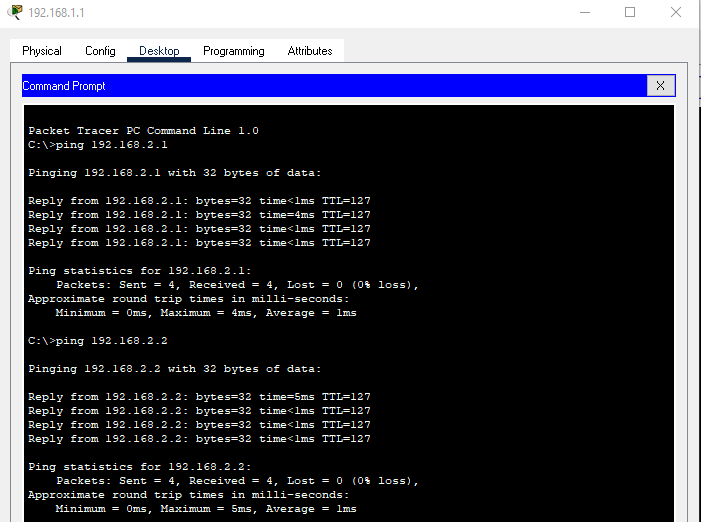
\includegraphics[width=\textwidth,height=.49\textwidth,keepaspectratio]{./img/test2.png}
    \caption{Vlan 10 mit Vlan 20}
\end{figure}
\begin{figure}[!htb]
    \centering
    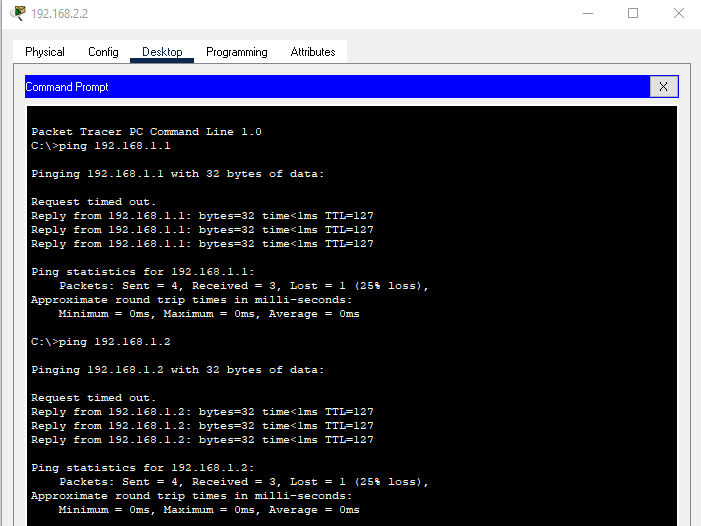
\includegraphics[width=\textwidth,height=.49\textwidth,keepaspectratio]{./img/test1.png}
    \caption{Vlan 20 mit Vlan 10}
    \caption{Config nach den Änderungen}
\end{figure}
\FloatBarrier
\subsubsection{Routerkommunikation}
\begin{figure}[!htb]
    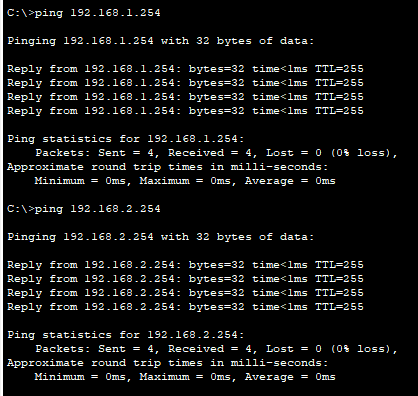
\includegraphics[width=\textwidth,height=\textwidth,keepaspectratio]{./img/ping_router.png}
    \caption{Ping zu den Subinterfaces}
\end{figure}
\pagebreak
\subsubsection{Frage 3}
\paragraph{Frage}
Wie könnte die Verbindung zwischen verschiedenen VLANs ohne eine
Router on a Stick Konfiguration hergestellt werden, und was würde sich ändern,
wenn die Switch keinen Trunk Port verwenden würde?
\paragraph{Antwort}
Man könnte die Verbindung zu den Endsystemen zu Trunk Port machen, aber das lässt sich nicht so einfach skalieren.\\
Wenn die Switches keinen Trunk Port verwenden dürfen, können die Geräte ohne Router nicht kommunizieren, da die Switches nur das eingestellte Access VLAN erlauben.